\subsection{
    Сумма и пересечение линейных подпространств.
}   

\begin{definition}
    Пусть $\mathcal{H}_1$ и $\mathcal{H}_2$ - линейные подпространства в линейном пространстве $\mathcal{L}$. Множество $\mathcal{H}_1 + \mathcal{H}_2$ всех векторов $\vec{x}$ вида $\vec{x} = \vec{x_1} + \vec{x_2}$, где $\vec{x_1} \in \mathcal{H}_1$, $\vec{x_2} \in \mathcal{H}_2$, называют \textbf{\textit{суммой линейных подпространств}} $\mathcal{H}_1$ и $\mathcal{H}_2$. 
\end{definition}

\begin{figure}[H]
    \centering
    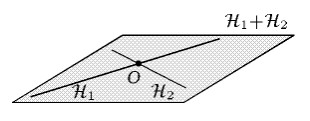
\includegraphics[scale=0.7]{images/module1/question04/1.jpg}
    \label{fig:picture_04_1}
    \caption{Сумма линейных подпространств.}
\end{figure}

\begin{definition}
    Пусть $\mathcal{H}_1$ и $\mathcal{H}_2$ - линейные подпространства в линейном пространстве $\mathcal{L}$. Множество $\mathcal{H}_1 \cap \mathcal{H}_2$ всех векторов $\vec{x}$, где $\vec{x} \in \mathcal{H}_1$ и $\vec{x} \in \mathcal{H}_2$, называют \textbf{\textit{пересечением линейных подпространств}} $\mathcal{H}_1$ и $\mathcal{H}_2$.
\end{definition}

\begin{figure}[H]
    \centering
    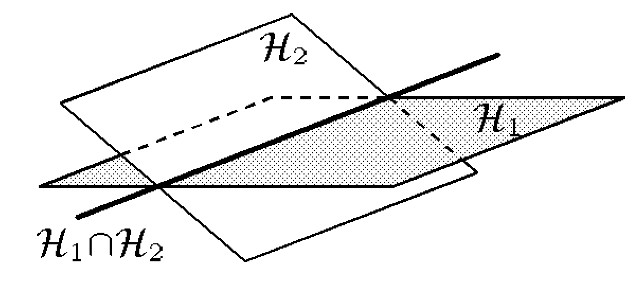
\includegraphics[scale=0.4]{images/module1/question04/2.jpg}
    \label{fig:picture_04_2}
    \caption{Пересечение линейных подпространств.}
\end{figure}

